% !TeX root = ./9-handout.tex

\setcounter{section}{8}

\section{Semantics of QL}

\begin{frame}
%\large

\scriptsize{\tableofcontents}

\end{frame}

\subsection{Arguments and validity in QL}

\begin{frame}
  \frametitle{Validity of arguments}

Valid? 

  \begin{earg}
    \item[] Everyone is either good or evil.
    \item[] Not everyone is a villain.
    \item[] Only villains are evil.
    \item[\therefore] Some heroes are good.
  \end{earg}

\end{frame}

\begin{frame}
\frametitle{Validity in QL}

\begin{itemize}[<+->]
\item Want to capture validity \emph{in virtue of the meanings of the
  connectives and the quantifiers} \\ (but ignoring the meanings of predicate
  symbols)
\item So we want to ignore any restrictions the predicate symbols place on their \emph{extensions}
\item Hence: allow \emph{any} extension in a potential counterexample
\item An argument is \emph{QL-valid} if there is \emph{no interpretation} in which the premises are true and the conclusion false
\end{itemize}
\end{frame}


\begin{frame}
\frametitle{Forms of arguments}

\begin{earg}
  \item[] Everyone is either good or evil.
  \item[] Not everyone is a villain.
  \item[] Only villains are evil.
  \item[\therefore] Some heroes are good.
\end{earg}

\begin{earg}
\item[] $\qt{\forall}{x}( G\qv{x} \eor  E\qv{x})$
\item[] $\enot \qt{\forall}{x}\, V\qv{x}$
\item[] $\qt{\forall}{x} (E\qv{x} \eif V\qv{x})$
\item[\therefore] $\qt{\exists}{x} (H\qv{x} \eand G\qv{x})$
\end{earg}

\end{frame}


\begin{frame}
\frametitle{(In)validity of arguments}

\begin{earg}
\item[] $\qt{\forall}{x}( G\qv{x} \eor  E\qv{x})$
\item[] $\enot \qt{\forall}{x}\, V\qv{x}$
\item[] $\qt{\forall}{x} (E\qv{x} \eif V\qv{x})$
\item[\therefore] $\qt{\exists}{x} (H\qv{x} \eand G\qv{x})$
\end{earg}

\begin{ekey}
\item[$Domain$] the inner planets (Mecury, Venus, Mars, Earth)
\item[G\qv{x}] $x$ is smaller than Earth
\item[E\qv{x}] $x$ is inhabited
\item[V\qv{x}] $x$ has a moon
\item[H\qv{x}] $x$ has rings
\end{ekey}
\end{frame}

\subsection{Interpretations}

\begin{frame}
\frametitle{Interpretations}

\begin{itemize}[<+->]
\item Domain: collection of objects (not empty)
\item \emph{Referents} for each name (which object it names)
\item Properties of each object
  \begin{itemize}
  \item \emph{Extension} of each 1-place predicate symbol: \\ \phantom{\emph{Extension}} the set of objects it applies to
  \end{itemize}
  \bigskip
\item Relations between each pair of objects
\begin{itemize}
\item \emph{Extension} of each $2$-place predicate symbol: \\ \phantom{\emph{Extension}} all pairs of
  objects standing in that relation
\end{itemize}
\end{itemize}

\end{frame}

\begin{frame}
\frametitle{Extensions}

\begin{ekey}
  \item[$Domain$] the inner planets
  \item[G\qv{x}] $x$ is smaller than Earth
  \item[E\qv{x}] $x$ is inhabited
  \item[V\qv{x}] $x$ has a moon
  \item[H\qv{x}] $x$ has rings
\end{ekey}

\begin{ekey}
\item[$Domain$] Mercury, Venus, Earth, Mars
\item[G\qv{x}] Mercury, Venus, Mars
\item[E\qv{x}] Earth
\item[V\qv{x}] Earth, Mars
\item[H\qv{x}] ---
\end{ekey}
\end{frame}

\begin{frame}
  \frametitle{(In)validity of arguments}

\begin{earg}
\item[] $\qt{\forall}{x}( G\qv{x} \eor  E\qv{x})$
\item[] $\enot \qt{\forall}{x}\, V\qv{x}$
\item[] $\qt{\forall}{x} (E\qv{x} \eif V\qv{x})$
\item[\therefore] $\qt{\exists}{x} (H\qv{x} \eand G\qv{x})$
\end{earg}

\begin{ekey}
\item[$Domain$] Mercury, Venus, Earth, Mars
\item[G\qv{x}] Mercury, Venus, Mars
\item[E\qv{x}] Earth
\item[V\qv{x}] Earth, Mars
\item[H\qv{x}] ---
\end{ekey}
\end{frame}

\begin{frame}
\frametitle{(In)validity of arguments}

\begin{earg}
\item[] $\qt{\forall}{x}( G\qv{x} \eor  E\qv{x})$
\item[] $\enot \qt{\forall}{x}\, V\qv{x}$
\item[] $\qt{\forall}{x} (E\qv{x} \eif V\qv{x})$
\item[\therefore] $\qt{\exists}{x} (H\qv{x} \eand G\qv{x})$
\end{earg}

\begin{ekey}
\item[$Domain$] $1$, $2$, $3$, $4$
\item[G\qv{x}] $1$, $2$, $4$
\item[E\qv{x}] $3$
\item[V\qv{x}] $3$, $4$
\item[H\qv{x}] ---
\end{ekey}
\end{frame}

\begin{frame}
  \frametitle{(In)validity of arguments}
  
  \begin{earg}
  \item[] $\qt{\forall}{x}( G\qv{x} \eor  E\qv{x})$
  \item[] $\enot \qt{\forall}{x}\, V\qv{x}$
  \item[] $\qt{\forall}{x} (E\qv{x} \eif V\qv{x})$
  \item[\therefore] $\qt{\exists}{x} (H\qv{x} \eand G\qv{x})$
  \end{earg}
  
  \begin{ekey}
  \item[$Domain$] $1$
  \item[G\qv{x}] $1$
  \item[E\qv{x}] ---
  \item[V\qv{x}] ---
  \item[H\qv{x}] ---
  \end{ekey}
  \end{frame}

\begin{frame}
\frametitle{Extensions of predicates}

\begin{ekey}
\item[$Domain$] $1$, $2$, $3$
\item[P\qv{x}] $1$, $2$
\item[Q\qv{x}] $2$, $3$
\item[R\qv{x}] ---
\end{ekey}

\hfill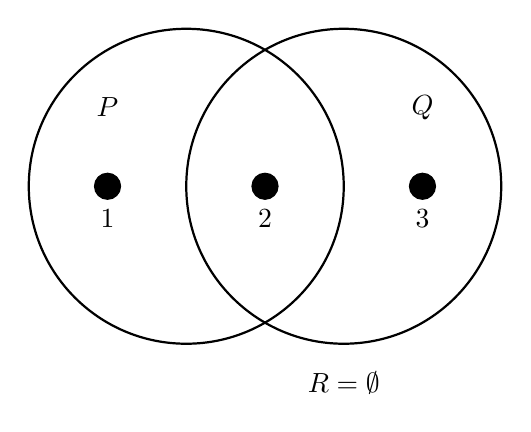
\begin{tikzpicture}
\def\circleA{(0,0) circle (2cm)}
\def\circleB{(0:2cm) circle (2cm)}
		%\begin{scope}
		%\clip \circleA;
		%\clip \circleB;
		%\fill[red!50] \circleA;
		%\end{scope}
		\draw[thick] \circleA;
    \node at (-1,1) {$P$};
    \node at (3,1) {$Q$};
    \node at (2,-2.5) {$R = \emptyset$};
		\draw[thick] \circleB;
    \node[circle,fill,draw,label={below:$1$}] at (-1,0) {};
    \node[circle,fill,draw,label={below:$2$}] at (1,0) {};
    \node[circle,fill,draw,label={below:$3$}] at (3,0) {};
\end{tikzpicture}
\end{frame}

\begin{frame}
\frametitle{(In)validity of arguments}

\begin{earg}
\item[] $\qt{\forall}{x}(G\qv{x} \eor E\qv{x})$
\item[] $\enot \qt{\forall}{x}\, V\qv{x}$
\item[] $\qt{\forall}{x} (E\qv{x} \eif V\qv{x})$
\item[\therefore] $\qt{\exists}{x} (H\qv{x} \eand G\qv{x})$
\end{earg}

\begin{ekey}
\item[$Domain$] $1$, $2$
\item[G\qv{x}] $1$
\item[E\qv{x}] $2$
\item[V\qv{x}] $2$
\item[H\qv{x}] $2$
\end{ekey}

\vspace{-3cm}\hfill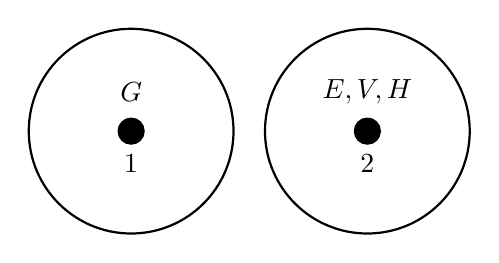
\begin{tikzpicture}
    \node at (-1.5,.5) {$G$};
    \node at (1.5,.5) {$E, V, H$};
		\draw[thick] (1.5,0) circle (1.3cm);
    \draw[thick] (-1.5,0) circle (1.3cm);
    \node[circle,fill,draw,label={below:$1$}] at (-1.5,0) {};
    \node[circle,fill,draw,label={below:$2$}] at (1.5,0) {};
\end{tikzpicture}

\end{frame}


\begin{frame}
\frametitle{Extensions of predicates}

\begin{ekey}
\item[$Domain$] $1$, $2$, $3$
\item[$a$] $1$
\item[A\qr{x}{y}] $\langle 1, 1\rangle$, $\langle 1,2\rangle$, $\langle 1,3\rangle$, $\langle 2,3\rangle$
\end{ekey}
\usetikzlibrary{arrows}
\hfill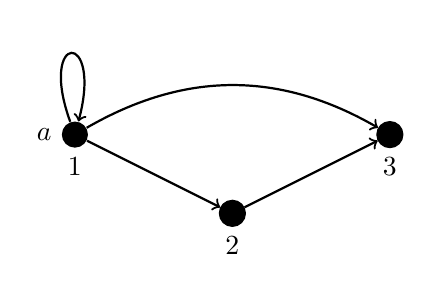
\begin{tikzpicture}
    \node[circle,fill,label={below:$1$},label={left:$a$}] (A) at (-1,0) {};
    \node[circle,fill,draw,label={below:$2$}] (B) at (1,-1) {};
    \node[circle,fill,draw,label={below:$3$}] (C) at (3,0) {};
    \draw[->,thick] (A) to[loop above,looseness=30,out=110] (A);
    \draw[->,thick] (A) -- (B);
    \draw[->,thick] (A) to[bend left] (C);
    \draw[->,thick] (B) -- (C);
\end{tikzpicture}
\end{frame}

\subsection{Truth of sentences of QL}

\begin{frame}
  \frametitle{Truth of sentences of QL}

  \begin{itemize}[<+->]
    \item Given an interpretation $I$ \dots
    \item An \emph{atomic sentence} is true iff the referents of the constants are in the extension of the predicate:
    \begin{itemize}
    \item $P\qv{a}$ is true iff referent `$r$' of $a$ is in extension of $P$
    \item $R\qr{a}{b}$ is true iff $\langle r,p\rangle$ is in extension of $R$\\
    (where $r$ is referent of $a$, and $p$ is referent of $b$)
    \end{itemize}
    \item $\enot\metav{A}$ is true iff $\metav{A}$ is false
    \item $\metav{A} \eor \metav{B}$ is true iff at least one of $\metav{A}$, $\metav{B}$ is true
    \item $\metav{A} \eand \metav{B}$ is true iff both $\metav{A}$, $\metav{B}$ are true
    \item $\metav{A} \eif \metav{B}$ is true iff $\metav{A}$ is false or $\metav{B}$ is true
  \end{itemize}
\end{frame}

\begin{frame}
  \frametitle{Truth of quantified sentences}

  \begin{itemize}[<+->]
    \item $\qt{\exists}{x}\,\metav{A}\qv{x}$ is true iff $\metav{A}\qv{x}$ is \emph{satisfied} by \emph{at least one} object in the domain
    \begin{itemize}
    \item $r$ satisfies $\metav{A}\qv{x}$ in $I$ iff $\metav{A}\qv{r}$ is true in the interpretation 
     %following perhaps has a typo: \item $o$ satisfies $\metav{A}\qv{x}$ iff $\metav{A}\qv{c}$ is true in interpretation just like $I$, but with $o$ as referent of $c$
    \end{itemize}
    \bigskip
    
    \item $\qt{\forall}{x}\,\metav{A}\qv{x}$ is true iff $\metav{A}\qv{x}$ is \emph{satisfied} by \emph{every} object in the domain
  \end{itemize}
\end{frame}

\begin{frame}
  \frametitle{Truth of quantified sentences}
\large 
  \begin{itemize}[<+->]
    \item $\qt{\exists}{x}\,(\metav{A}\qv{x} \eand \metav{B}\qv{x})$ is true iff \textcolor{OGlyallpink}{some} object satisfies `$\metav{A}\qv{x} \eand \metav{B}\qv{x}$'
    \begin{itemize}
      \item $o$ satisfies `$\metav{A}\qv{x} \eand \metav{B}\qv{x}$' iff it satisfies both $\metav{A}\qv{x}$ and $\metav{B}\qv{x}$
    \end{itemize}
    
\bigskip

    \item $\qt{\forall}{x}\,(\metav{A}\qv{x} \eif \metav{B}\qv{x})$ is true iff \emph{every} object satisfies `$\metav{A}\qv{x} \eif \metav{B}\qv{x}$'
    \medskip
    \begin{itemize} 
    \large 
      \item $o$ satisfies `$\metav{A}\qv{x} \eif \metav{B}\qv{x}$' iff
      either
      \bigskip
      \begin{itemize}  
      \normalsize
        \item $o$ does not satisfy $\metav{A}\qv{x}$ (vacuously true conditional)
        \item[] \makebox[\textwidth]{or}
        \item $o$ does satisfy $\metav{B}\qv{x}$
      \end{itemize}
       \bigskip
    \end{itemize}
  \end{itemize}
\end{frame}


\begin{frame}
\frametitle{Making ``Some $A$s are $B$s'' true}

\begin{columns}
  \begin{column}{.5\textwidth}

%\begin{multicols}{2}

    \begin{itemize}
      \item $\qt{\exists}{x}\,(A\qv{x} \eand B\qv{x})$
      \item Extension of $A$ and $B$ must have something in common.
      \item[] (Filled area must contain at least one object)
      \item $A$ and $B$ can \alert<1>{overlap}, \alert<2>{be equal}, or \alert<3->{be contained}.
      \item Same situations make \\ ``No $A$s are $B$s'' \emph{false}.
    \end{itemize}
 \end{column}
  
 % \columnbreak
 
 %JH: to get the individual slide frames to render in the handout mode, use following code:
% \only<1| handout:1>{text1}
% explained at bottom here: https://tex.stackexchange.com/questions/183093/beamer-handout-mode-explicitly-printing-half-way-frames
  
 \begin{column}{.5\textwidth}
\only<1| handout:1>{\begin{tikzpicture}
\def\circleA{(0,0) circle (1.5cm)}
\def\circleB{(0:1.5cm) circle (1.5cm)}
		\begin{scope}
		\clip \circleA;
		\clip \circleB;
		\fill[highlightbg] \circleA;
		\end{scope}
		\draw[thick] \circleA;
    \node at (-1,.5) {$A$};
    \node at (2.5,.5) {$B$};
		\draw[thick] \circleB;
\end{tikzpicture}}
\only<3| handout:3>{\begin{tikzpicture}
  \def\circleA{(0,0) circle (2cm)}
  \def\circleB{(0:.5cm) circle (1cm)}
      \begin{scope}
      \clip \circleA;
      \clip \circleB;
      \fill[highlightbg] \circleA;
      \end{scope}
      \draw[thick] \circleA;
      \node at (-1,1) {$A$};
      \node at (0,.5) {$B$};
      \draw[thick] \circleB;
  \end{tikzpicture}}
\only<2| handout:2>{\begin{tikzpicture}
  \def\circleA{(0,0) circle (2cm)}
  \def\circleB{(0:.5cm) circle (1cm)}
      %\begin{scope}
      %\clip \circleA;
      %\clip \circleB;
      %\fill[highlightbg] \circleA;
      %\end{scope}
      \draw[thick,fill=highlightbg] \circleA;
      %\node at (-1,1) {};
      \node at (0,.5) {$A = B$};
      %\draw[thick] \circleB;
  \end{tikzpicture}}
  \only<4| handout:4>{\begin{tikzpicture}
    \def\circleA{(0,0) circle (2cm)}
    \def\circleB{(0:.5cm) circle (1cm)}
        \begin{scope}
        \clip \circleA;
        \clip \circleB;
        \fill[highlightbg] \circleA;
        \end{scope}
        \draw[thick] \circleA;
        \node at (-1,1) {$B$};
        \node at (0,.5) {$A$};
        \draw[thick] \circleB;
    \end{tikzpicture}}
\end{column}
\end{columns}

%\end{multicols}
\end{frame}

\begin{frame}
\frametitle{Making ``Some $A$s are $B$s'' false}

\begin{columns}
  \begin{column}{.5\textwidth}
    \begin{itemize}
      \item $\enot\qt{\exists}{x}\,(A\qv{x} \eand B\qv{x})$
      \item Extension of $A$ and $B$ must have nothing in common.
      \item $A$ and $B$ \alert<1>{don't overlap}, or \alert<2,3>{one} or \alert<4>{both} \alert<2->{empty}.
      \item Same situations make \\``No $A$s are $B$s'' \emph{true}.
    \end{itemize}
  \end{column}
  \begin{column}{.5\textwidth}
\only<1| handout:1>{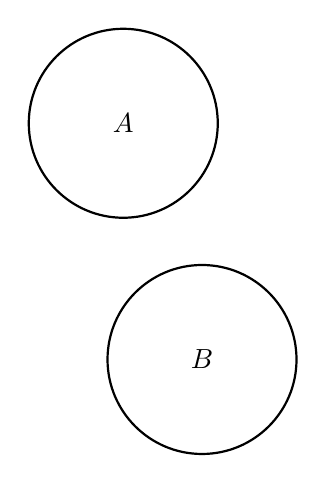
\begin{tikzpicture}
\def\circleA{(1,0) circle (1.2cm)}
\def\circleB{(0,3) circle (1.2cm)}
		\draw[thick] \circleA;
    \node at (1,0) {$B$};
    \node at (0,3) {$A$};
		\draw[thick] \circleB;
\end{tikzpicture}}
\only<2| handout:2>{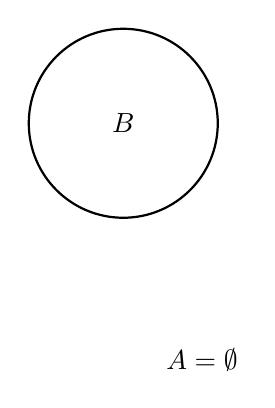
\begin{tikzpicture}
  \def\circleA{(1,0) circle (1.2cm)}
  \def\circleB{(0,3) circle (1.2cm)}
      %\draw[thick] \circleA;
      \node at (1,0) {$A=\emptyset$};
      \node at (0,3) {$B$};
      \draw[thick] \circleB;
  \end{tikzpicture}}
\only<3| handout:3>{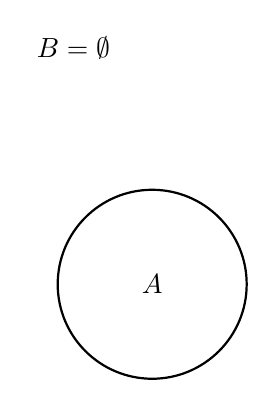
\begin{tikzpicture}
\def\circleA{(1,0) circle (1.2cm)}
\def\circleB{(0,3) circle (1.2cm)}
		\draw[thick] \circleA;
    \node at (1,0) {$A$};
    \node at (0,3) {$B=\emptyset$};
		%\draw[thick] \circleB;
\end{tikzpicture}}
\only<4| handout:4>{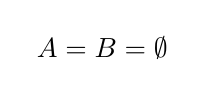
\begin{tikzpicture}
  %\def\circleA{(1,0) circle (1.2cm)}
  %\def\circleB{(0,3) circle (1.2cm)}
  %    \draw[thick] \circleA;
  %    \node at (1,0) {$A$};
      \node at (0,3) {$A= B=\emptyset$};
      %\draw[thick] \circleB;
  \end{tikzpicture}}
\end{column}
\end{columns}
\end{frame}

\begin{frame}
\frametitle{Making ``All $A$s are $B$s'' true}

\begin{columns}
  \begin{column}{.5\textwidth}
    \begin{itemize}
      \item $\qt{\forall}{x}\,(A\qv{x} \eif B\qv{x})$
      \item Extension of $A$ must be \alert<1>{contained in extension of $B$}.
      \item Extensions of $A$ and $B$ \alert<2>{can be the same}.
      \item Extension of $A$ \alert<3>{can be empty}.
      \item Same situations make \dots
      \begin{itemize}
        \item ``Only $B$s are $A$s'' \emph{true}.
        \item ``Some $A$s are not $B$s'' \emph{false}.
      \end{itemize}
    \end{itemize}
  \end{column}
  \begin{column}{.5\textwidth}
\only<1| handout:1>{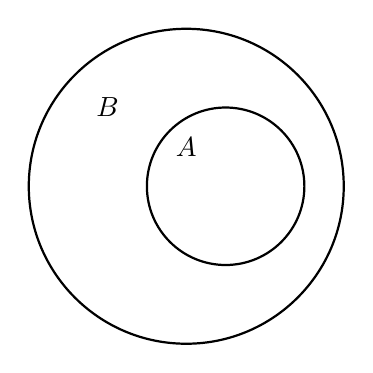
\begin{tikzpicture}
  \def\circleA{(0,0) circle (2cm)}
  \def\circleB{(0:.5cm) circle (1cm)}
      %\begin{scope}
      %\clip \circleA;
      %\clip \circleB;
      %\fill \circleA;
      %\end{scope}
      \draw[thick] \circleA;
      \node at (-1,1) {$B$};
      \node at (0,.5) {$A$};
      \draw[thick] \circleB;
  \end{tikzpicture}}
\only<2| handout:2>{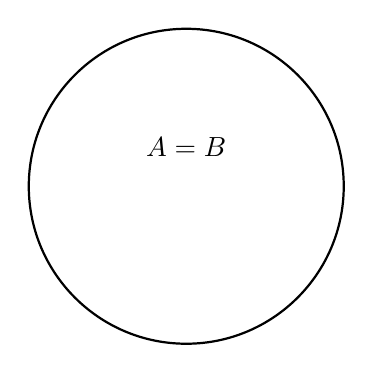
\begin{tikzpicture}
  \def\circleA{(0,0) circle (2cm)}
  \def\circleB{(0:.5cm) circle (1cm)}
      %\begin{scope}
      %\clip \circleA;
      %\clip \circleB;
      %\fill[highlightbg] \circleA;
      %\end{scope}
      \draw[thick] \circleA;
%      \node at (-1,1) {$B=A$};
      \node at (0,.5) {$A=B$};
      %\draw[thick] \circleB;
  \end{tikzpicture}}
\only<3| handout:3>{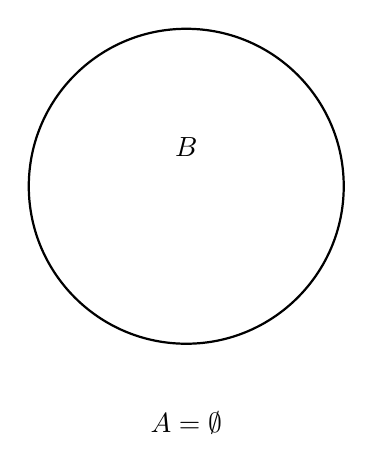
\begin{tikzpicture}
  \def\circleA{(0,0) circle (2cm)}
  \def\circleB{(0:.5cm) circle (1cm)}
      %\begin{scope}
      %\clip \circleA;
      %\clip \circleB;
      %\fill[highlightbg] \circleA;
      %\end{scope}
      \draw[thick] \circleA;
      \node at (0,.5) {$B$};
      \node at (0,-3) {$A=\emptyset$};
      %\draw[thick] \circleB;
  \end{tikzpicture}}
\end{column}
\end{columns}
\end{frame}

\begin{frame}
\frametitle{Making ``All $A$s are $B$s'' false}

\begin{columns}
  \begin{column}{.5\textwidth}
    \begin{itemize}
      \item $\qt{\forall}{x}\,(A\qv{x} \eif B\qv{x})$
      \item Extension of $A$ must \alert<1,2>{contain something not in} $B$.
      \item Extensions of $A$ \alert<3>{cannot be empty, but $B$ may be empty}.
      \item Same situations make \dots
    \begin{itemize}
        \item ``Only $B$s are $A$s'' \emph{false}.
        \item ``Some $A$s are not $B$s'' \emph{true}.
      \end{itemize}
    \end{itemize}
  \end{column}
  \begin{column}{.5\textwidth}
\only<1| handout:1>{\begin{tikzpicture}
\def\circleA{(0,0) circle (1.5cm)}
\def\circleB{(0:1.5cm) circle (1.5cm)}
		\begin{scope}[even odd rule]
		\clip \circleB (0,0) circle (2cm);
		\fill[highlightbg] \circleA;
		\end{scope}
		\draw[thick] \circleA;
    \node at (-1,.5) {$A$};
    \node at (2.5,.5) {$B$};
		\draw[thick] \circleB;
\end{tikzpicture}}
\only<2| handout:2>{\begin{tikzpicture}
\def\circleA{(1,0) circle (1.2cm)}
\def\circleB{(0,3) circle (1.2cm)}
		\draw[thick] \circleA;
		\draw[thick,fill=highlightbg] \circleB;\node at (1,0) {$B$};\node at (0,3) {$A$};
\end{tikzpicture}}
\only<3| handout:3>{\begin{tikzpicture}
\def\circleA{(0,0) circle (1.5cm)}
\def\circleB{(0:1.5cm) circle (1.5cm)}
		\begin{scope}
		\fill[highlightbg] \circleA;
		\end{scope}
		\draw[thick] \circleA;
    \node at (-1,.5) {$A$};
    \node at (2.5,.5) {$B=\emptyset$};
\end{tikzpicture}}
\end{column}
\end{columns}
\end{frame}


\subsection{Testing for validity}

\begin{frame}
\frametitle{Arguments involving quantifiers}

\begin{enumerate}[<+->]
\item If an action x is morally wrong then
A is blameworthy for freely doing x.
\item If x is rationally optimal (there is no action which A has
  reason to think there is more reason for A to do), then A is not
  blameworthy for freely doing x.
\item Therefore, if x is morally wrong, then
x is not rationally optimal.
(Principle of moral categoricity.)
\end{enumerate}

\begin{raggedleft}
\small--John Skorupski, \textit{Ethical Explorations}, 2000 (\href{http://books.google.com/books?id=bxIzZYqRZdwC&lpg=PP1&pg=PA170\#v=onepage&q&f=false}{link})
 \end{raggedleft}

\end{frame}

\begin{frame}
  \frametitle{Symbolizing Skorupski}

  \begin{enumerate}
    \only<1-2>{\item[1.] If an action x is morally wrong then
    A is blameworthy for freely doing x.}
    \only<3-4>{\item[2.] If x is rationally optimal, then A is not
      blameworthy for freely doing x.}
    \only<5-6>{\item[3.] Therefore, if x is morally wrong, then
    x is not rationally optimal. }
    \end{enumerate}

  \begin{ekey}
  \item[$Domain$] actions
  \item[W\qv{x}] $x$ is morally wrong
  \item[B\qv{x}] A is blameworthy for freely doing $x$
  \item<3->[O\qv{x}] $x$ is rationally optimal
  \end{ekey}
  \begin{earg}
  \item<1->[] \uncover<2->{\alert<2>{$\qt{\forall}{x}(W\qv{x} \eif B\qv{x})$}}
  \item<3->[] \uncover<4->{\alert<4>{$\qt{\forall}{x}(O\qv{x} \to \lnot B\qv{x})$}}
  \item<5->[\therefore] \uncover<6>{\alert<6>{$\qt{\forall}{x}(W\qv{x} \to \lnot O\qv{x})$}}
  \end{earg}

  \end{frame}

\begin{frame}
\frametitle{Symbolizing Skorupski}

\begin{ekey}
\item[$Domain$] actions
\item[W\qv{x}] $x$ is morally wrong
\item[B\qv{x}] A is blameworthy for freely doing $x$
\item[O\qv{x}] $x$ is rationally optimal
\end{ekey}
\begin{earg}
\item[] $\qt{\forall}{x}(W\qv{x} \eif B\qv{x})$
\item[] $\qt{\forall}{x}(O\qv{x} \to \lnot B\qv{x})$
\item[\therefore] $\qt{\forall}{x}(W\qv{x} \to \lnot O\qv{x})$
\end{earg}

\begin{earg}
\item[] All Ws are Bs
\item[] No Os are Bs (iff No Bs are Os)
\item[\therefore] No Ws are Os
\end{earg}

\end{frame}

\begin{frame}{Determining validity}

  \begin{columns}
    \begin{column}{.5\textwidth}
      \begin{itemize}[<+->]
        \item Make conclusion $\qt{\forall}{x}(W\qv{x} \to \lnot O\qv{x})$ false.
        \item Make $\qt{\exists}{x}(W\qv{x} \land O\qv{x})$ true.
        \item Make $\qt{\forall}{x}(W\qv{x} \eif B\qv{x})$ true.
        \item $\qt{\exists}{x}(O\qv{x} \land B\qv{x})$ is now forced to be true.
        \item So, $\qt{\forall}{x}(O\qv{x} \to \lnot B\qv{x})$ is false.
        \item But those are not the only possibilities!
      \end{itemize}
    \end{column}
    \begin{column}{.5\textwidth}
\only<2->{\begin{tikzpicture}
  \def\circleA{(0,0) circle (1.5cm)}
  \def\circleB{(0:1.5cm) circle (1.5cm)}
  \def\circleC{(0,0) circle (2.3cm)}
      \begin{scope}
      \clip \circleA;
      \clip \circleB;
      \fill[highlightbg] \circleA;
      \end{scope}
      \draw[thick] \circleA;
      \node at (-1,.5) {$W$};
      \node at (2.5,.5) {$O$};
      \draw[thick] \circleB;
      \uncover<3->{\draw[thick] \circleC;
      \node at (-1.7,.5) {$B$};}
\end{tikzpicture}}
\end{column}
\end{columns}
\end{frame}

\begin{frame}{Other configurations}
  \begin{columns}
  \begin{column}{.4\textwidth}
  \begin{tikzpicture}
    \def\circleA{(0,0) circle (1.5cm)}
    \def\circleB{(0:1.5cm) circle (1.5cm)}
    \def\circleC{(.6,0) circle (2.8cm)}
        \begin{scope}
        \clip \circleA;
        \clip \circleB;
        \fill[highlightbg] \circleA;
        \end{scope}
        \draw[thick] \circleA;
        \node at (-1,.5) {$W$};
        \node at (2.5,.5) {$O$};
        \draw[thick] \circleB;
        \draw[thick] \circleC;
        \node at (-1.7,.5) {$B$};
  \end{tikzpicture}
\end{column}
\begin{column}{.6\textwidth}
  \vspace*{2ex}
  
  \begin{tikzpicture}
    \def\circleA{(0,0) circle (1.5cm)}
    \def\circleB{(0:1.5cm) circle (1.5cm)}
        \begin{scope}
        \clip \circleA;
        \clip \circleB;
        \fill[highlightbg] \circleA;
        \end{scope}
        \draw[thick] \circleA;
        \node at (-.8,0) {$W = B$};
        \node at (2.5,0) {$O$};
        \draw[thick] \circleB;
  \end{tikzpicture}
\\[-2ex]
\hfill\begin{tikzpicture}
    \def\circleA{(0,0) circle (1cm)}
    \def\circleC{(0,0) circle (2cm)}
        \fill[highlightbg] \circleA;
        \draw[thick] \circleA;
        \node at (0,0) {$W = O$};
        \draw[thick] \circleC;
        \node at (-1.5,0) {$B$};
  \end{tikzpicture}
\end{column}
\end{columns}
\end{frame}

\subsection{Semantic notions in QL}

\begin{frame}
\frametitle{Semantics notions in QL}

%$\boldsymbol\models$

\begin{itemize}[<+->]
  \item $\metav{P}_1,\dots,\metav{P}_n \mathrel{\emph{\entails}} \metav{Q}$ if no interpretation
  makes all of $\metav{P}_1,\dots,\metav{P}_n$ true and $\metav{Q}$~false.
  \item $\metav{P}$ is a \emph{validity} ($\entails \metav{P}$) if it is true in every interpretation.
  \item $\metav{P}$ and $\metav{Q}$ are \emph{equivalent in QL} if no
 interpretation makes one true but the other false.
 \item $\metav{P}_1,\dots,\metav{P}_n$ are \emph{jointly satisfiable
 in QL} if some interpretation makes all of them true %at the same time.
\end{itemize}
\end{frame}

\begin{frame}
\frametitle{Using interpretations}

\begin{itemize}[<+->]
\item By providing one suitable interpretation we \emph{can} show that\dots
\begin{itemize}[<+->]
  \item an argument is \emph{not valid} in QL
  \item a sentence is \emph{not a validity} in QL
  \item two sentences are \emph{not equivalent} in QL
  \item some sentences \emph{are satisfiable} in QL
\end{itemize}
\item But we \emph{cannot} show using any number of interpretations that\dots
\begin{itemize}[<+->]
  \item an argument \emph{is valid} in QL
  \item a sentence \emph{is a validity} in QL
  \item two sentences \emph{are equivalent} in QL
  \item some sentences \emph{are not satisfiable} in QL
\end{itemize}
\end{itemize}
\end{frame}

\begin{frame}
\frametitle{Examples}

\begin{itemize}[<+->]
  \item $\qt{\forall}{x}(A\qv{x} \eor B\qv{x})$ and $\qt{\forall}{x}\,A\qv{x} \eor \qt{\forall}{x}\,B\qv{x}$ are not equivalent.
  \item  $\qt{\forall}{x}(A\qv{x} \eif B\qv{x}), \qt{\forall}{x}(A\qv{x} \eif \enot B\qv{x})$ are jointly satisfiable.
  \item $\qt{\forall}{x}(\enot A\qv{x} \eif B\qv{x}), \qt{\exists}{x}(B\qv{x} \eand C\qr{x}{b})
  \nentails \qt{\exists}{x}(\enot A\qv{x} \eand C\qr{x}{b})$.
  \item $ \nentails \qt{\exists}{x}\, A\qr{a}{x} \eif \qt{\exists}{x}\, A\qr{x}{x}$.
\end{itemize}
Test solutions on \href{https://carnap.io/assignments/2022\%20Fall,\%2024.241\%20MIT\%20Logic\%201/Week\%209\%20PRACTICE\%20problems\%20for\%20QL\%20Models}{this week's practice problems}!

%\not\models

\end{frame}

\subsection{Arguing about interpretations}

\begin{frame}
\frametitle{Arguing about Interpretations}

\begin{itemize}[<+->]
  \item No interpretation(s) can show that an argument is valid.
  \item That's because there is no way to inspect all possible interpretations.
  \item But we can show that arguments are valid, by:
  \begin{itemize}
    \item a formal proof (a future topic!)
    \item an informal argument
  \end{itemize}
  \item The informal argument makes use of the \emph{truth conditions}
  for sentences of QL.
  \item Analogous to arguing about valuations in SL.
\end{itemize}

\end{frame}

\begin{frame}
  \frametitle{Example}

  \[(\qt{\forall}{x}\metav{A}\qv{x} \lor \qt{\forall}{x}\metav{B}\qv{x}) \entails \qt{\forall}{x}(\metav{A}\qv{x} \lor \metav{B}\qv{x})\]
  \begin{itemize}[<+->]
  \item Suppose an interpretation makes premise $\qt{\forall}{x}\,\metav{A}\qv{x}
  \lor \qt{\forall}{x}\,\metav{B}\qv{x}$ true.
  \item By truth conditions for $\lor$, it makes either $\qt{\forall}{x}\metav{A}\qv{x}$ or $\qt{\forall}{x}\metav{B}\qv{x}$ true.
  \item Suppose it's the first, i.e., $\qt{\forall}{x}\,\metav{A}\qv{x}$ is true.
    \begin{itemize}[<+->]
      \item By truth conditions for $\forall$, every object in the domain satisfies $\metav{A}\qv{x}$.
      \item By the truth conditions for $\lor$, every object satisfies $\metav{A}\qv{x} \lor \metav{B}\qv{x}$
      \item So, by the truth conditions for $\forall$, $\qt{\forall}{x}(\metav{A}\qv{x}
      \lor \metav{B}\qv{x})$ is true.
    \end{itemize}
  \item Suppose it's the second, i.e., $\qt{\forall}{x}\metav{B}\qv{x}$ is true: Similarly\dots
  \item These are the only possibilities: so any interpretation that makes the premise true must also make the conclusion true.
  \end{itemize}
\end{frame}






